


	Os algoritmos \textit{TextTiling} e \textit{C99} foram propostos para o inglês e sem domínio determinado, ou seja, a proposta inicial é trabalhar em qualquer texto nessa língua.
	A proposta desse trabalho é adaptá-los ao contexto das atas de reunião em português do Brasil. As subseções seguintes tratam das adaptações para esse nicho mais específico. A seção~\ref{sec:avaliacao} mostra a análise dos algoritmos adaptados.



\subsection{Préprocessamento}
	\label{subsec:preprocessamento}




	O texto a ser segmentado frequentemente é extraído de documentos em formatos como \textit{pdf} ou de processadores de texto. Após a extração, esse pode passar por processos de transformação os quais serão apresentados a seguir.

	A etapa de pre-processamento, em um documento contendo texto puro, acontece em dois passos principais. Primeiro elimina-se as palavras consideradas menos informativas, as quais são chamadas de \textit{stop words}, para isso, utiliza-se uma lista contendo 438 palavras. Em seguida, remove-se os sufixos das palavras restantes, mantendo apenas o radical da palavra. A Figura~\ref{fig:exemplopreprocessamento} mostra a etapa de pré-processamento em uma sentença em português.
	



  \begin{figure}[!h]
	\centering
	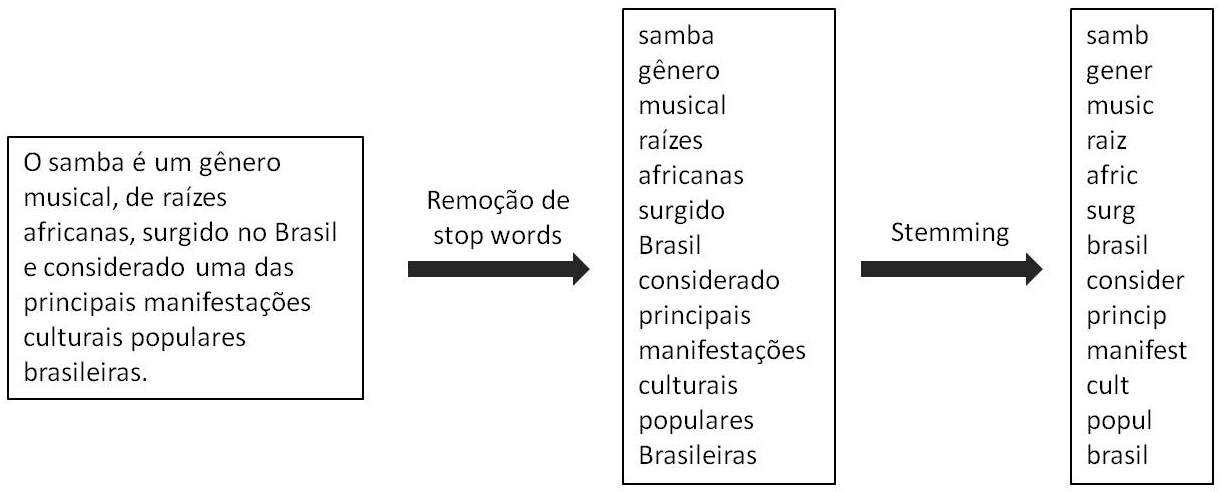
\includegraphics[width=0.45\textwidth]{exemplo-preprocessamento-noborder.jpg}
	\caption{Exemplo de pré-processamento}
	\label{fig:exemplopreprocessamento}
  \end{figure}


Há ainda outros passos presentes nessa etapa como remoção de acentos, transformações de caixa, remoção de pontuação, os quais são relativamente simples e não requerem maiores detalhes.





\subsubsection{Remoção de ruídos}

% Cabeçalhos e rodapés
As atas frequentemente contém trechos que podem ser considerados pouco informativos e descartados durante o pré-processamento. 
Após a extração, cabeçalhos e roda-pés se misturam aos tópicos tratados na reunião, podendo ser  inseridos no meio de um tópico e criando uma quebra que prejudica tanto o algoritmo de extração, quanto a leitura do texto pelo usuário.

% Numerais
Também é comum o uso de numerais para marcação de páginas e linhas, da mesma forma, são pouco informativos e podem ser removidos.

Nesse trabalho, esses elementos são removidos por meio de heurísticas simples, uma vez que, o descarte não causa perca de informação e pode facilitar a identificação dos segmentos, pois melhora a coesão do texto. Outro benefício é manter os segmentos livres de textos que fogem do assunto.


%Como forma de padronização, as instituições acrescentam ao documento

%		passos menores
%		1 - heurística simples para remover cabeçalho e rodapé.
%		2 - remoção de numerais
%		3 - remoção de acentos, transformações de caixa, remoção de pontuação.
		
	% Esses passos são realizados internamente em cada algorímo, para que a saida seja legível ao usuário final.





	

\subsection{Identificação de candidatos}
	\label{subsec:indentificacaosentencas}
	
%	Como entrada para os 
%	Os algoritmos de segmentação devem ser
	É preciso fornecer aos algoritmos os candidatos iniciais a limites de segmento. Aproveitando do estilo de escrita e baseando-se na pontuação do texto é possível indicar quebras de parágrafo, finais de sentenças ou mesmo palavras. 

	Ocorre que em atas de reunião é uma prática comum redigi-las de forma que o conteúdo discutido fica em parágrafo único, e quebras de parágrafo são usados para formatação de outros elementos como espaço para assinaturas. Indicar todo \textit{token} como ponto candidato obriga a ajustá-lo de maneira a não segmentar uma ideia ou frase. Assim, nesse trabalho, os finais de sentença são considerado candidatos passíveis a limite entre segmentos. 
	
	Devido ao estilo de pontuação desses documentos, como encerrar sentenças usando um \textit{";"} e inserção de linhas extras, usa-se as regras abaixo para identificar os finais de sentenças.  


\begin{algorithm}
	\SetKwInOut{Input}{Entrada}
	\SetKwInOut{Output}{Saída}
	\SetKwBlock{Inicio}{início}{fim}
	\SetKwFor{ParaTodo}{para todo}{}{fim para todo}
	\SetKwIF{Se}{SenaoSe}{Senao}{}{}{senao se}{senao}{fim se}
	\SetKwFor{Para}{}{}{}

	
	\Input{Texto}
	\Output{Texto com identificações de finais de sentença}
	
	\ParaTodo {token, marcá-lo como final de sentença se:} {	

	Terminar com um \texttt{!}\\
	Terminar com um \texttt{.} e não for uma abreviação\\
	Terminar em \texttt{.?;} e:
		\Para{}{
			For seguido de uma quebra de parágrafo ou tabulação\\
			O próximo \textit{token} iniciar com  \texttt{(\{["'}\\
			O próximo \textit{token} iniciar com letra maiúscula\\
			O penúltimo caracter  for \texttt{)\}]"'}\\
		}
	}
	
	\caption{Identificação de finais de sentença}
\end{algorithm}



%A qualidade do algoritmo é sempre dependente da escrita correta! Ausência de emoticons, códigos de computador e gírias.














